% !TEX encoding = UTF-8 Unicode
\chapter{Additional results and sensitivity analysis}     % numérotée
\label{chap-Annex}                   % étiquette pour renvois (à compléter!)

%\section{Algorithms} \label{sec:annex-alg-KF}
%
%\begin{itemize}
%	\item Multi-model algorithms MKF--SF and MKF--SP.  TODO: Not sure if this is needed...
%\end{itemize}

\section{Tuning of KF3 for MIMO linear system} \label{sec:annex-sim-2-KF-tuning}

As described in Chapter \ref{chap-simulation}, a standard Kalman filter was tuned to minimize the \gls{RMSE} of the output estimates using 5000 data samples from the $2\times2$ linear system. Since the system is symmetrical and the two \gls{RODD}s have the same parameters, it was assumed that the two observer parameters, $\sigma_{w_p,1,\text{opt}}$ and $\sigma_{w_p,2,\text{opt}}$ must also be identical. This assumption simplified the search process since only one optimum value needed to be found.

Figure \ref{fig:sim-sys-2x2-KF3-tuning-sens} shows the variation in the \gls{RMSE}s of the four model state estimates with different parameter values. Based on this, $\sigma_{w_p,1,\text{opt}}=\sigma_{w_p,2,\text{opt}}=0.01$ were chosen since this approximately minimizes the \gls{RMSE} of all the state estimates.
\begin{figure}[htp]
	\centering
	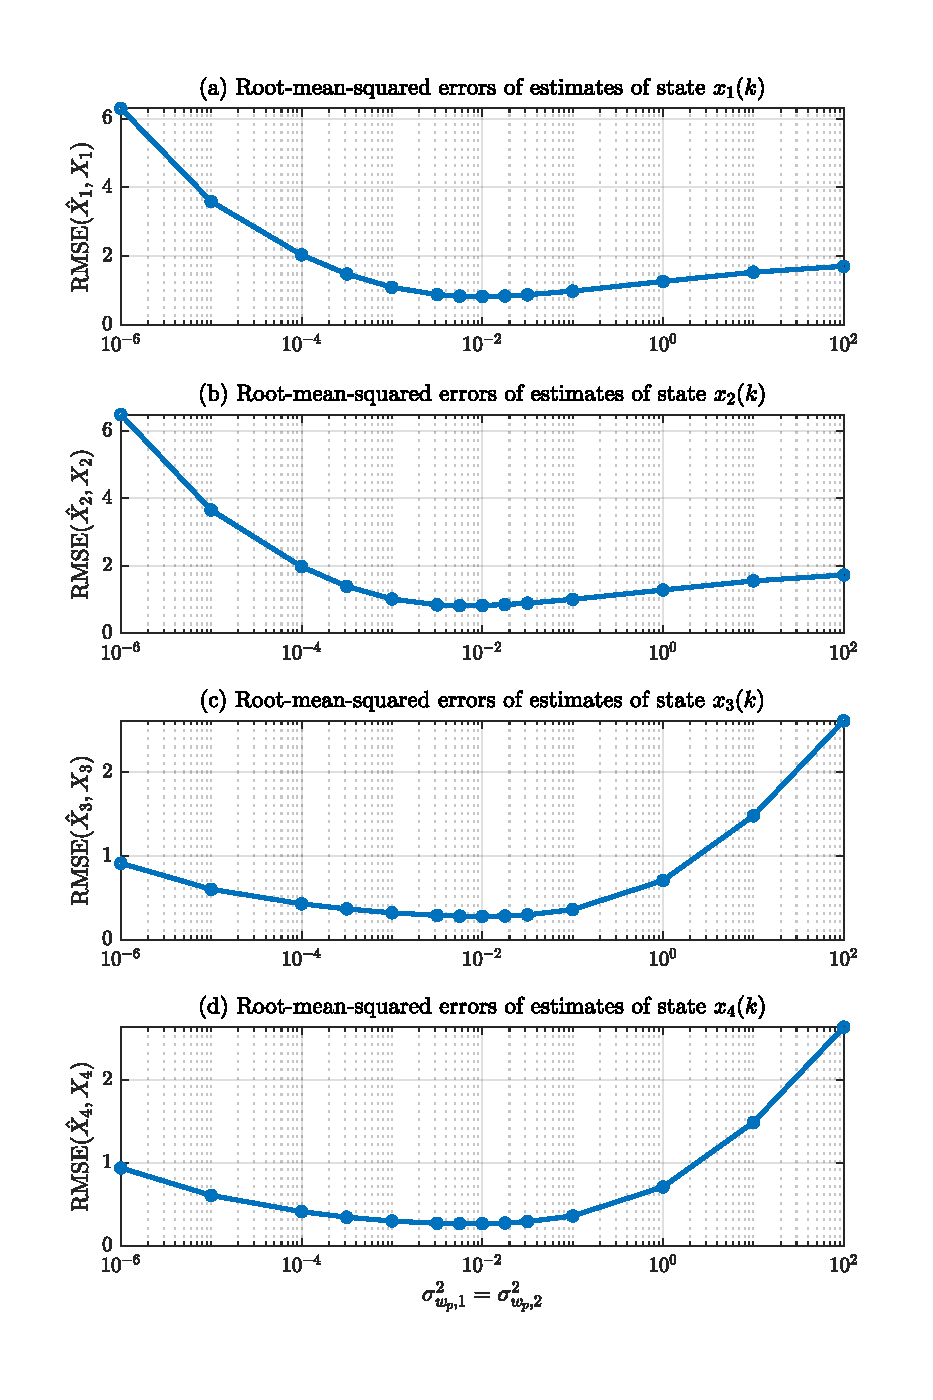
\includegraphics[width=14cm]{images/rod_obs_sim3_3KF_Q_seed_6.pdf}
	\caption{Tuning of Kalman filter KF3 – $2\times2$ system}
	\label{fig:sim-sys-2x2-KF3-tuning}
\end{figure}
Therefore the process noise covariance matrix of KF3 was
\begin{equation} \label{eq:sim-sys-sim3-KF3-Q}
	\begin{aligned}
		\mathbf{Q}_{\text{KF3}}=\mathbf{Q}_{\text{opt}}=\begin{bmatrix}
			\sigma_{x_1}^2 & 0 & 0 & 0 \\
			0 & \sigma_{x_2}^2 & 0 & 0 \\
			0 & 0 & \sigma_{w_p,1,\text{opt}}^2 & 0 \\
			0 & 0 & 0 & \sigma_{w_p,2,\text{opt}}^2
		\end{bmatrix}=\begin{bmatrix}
			0.1^2 & 0 & 0 & 0 \\
			0 & 0.1^2 & 0 & 0 \\
			0 & 0 & 0.1^2 & 0 \\
			0 & 0 & 0 & 0.1^2
		\end{bmatrix}.
	\end{aligned}
\end{equation}

\section{Tuning of MKF observers for MIMO linear system} \label{sec:annex-sim-2-MKF-tuning}

 In the case of the sequence fusion algorithm, the candidate parameter values were chosen from the same sets as those used for the \gls{SISO} system (\ref{eq:sim-sys-siso-MKF-SF-param-values}). Again, only observers with 200 hypotheses or less and a total hypothesis probability, $\beta$, greater than 0.85 were tested. For the selection of the sequence pruning algorithm parameters, the possible number of hypotheses was increased to 200 since it was expected to require more hypothesis sequences in the \gls{MIMO} experiment. The candidate values for the sequence pruning parameters were
\begin{equation} \label{eq:sim-sys-mimo-MKF-SP-param-values}
	\begin{aligned}
		n_h &\in \left\{ 24, 46, 68, 90, 112, 134, 156, 178, 200 \right\},  \\
		N_\text{min} &\in \left\{1, 2, 3, 4, 5, 6, 7, 9, 12, 16, 21\right\}.
	\end{aligned}
\end{equation}

As in the \gls{SISO} experiment, the resulting observers were simulated on a set of 5000 input-output samples from the simulated process (\ref{eq:sim-sys-mimo-ct}), and the \gls{RMSE}s calculated. Tables \ref{tb:obs-sim2-popt-SF95}, \ref{tb:obs-sim2-popt-SF98}, and \ref{tb:obs-sim2-popt-SP} show the results of the 10 best combinations of parameter values for the two sequence fusion algorithms (1995 and 1998 versions), and the sequence pruning algorithm.
\begin{table}[hb]
	\begin{center}
		\caption{Multi-model observer parameter search results – MKF--SF95.} \label{tb:obs-sim2-popt-SF95}
		% See: https://texblog.org/2019/06/03/control-the-width-of-table-columns-tabular-in-latex/
		\begin{tabular}{p{0.05\textwidth}>{\centering\arraybackslash}p{0.07\textwidth}>{\centering\arraybackslash}p{0.07\textwidth}>{\centering\arraybackslash}p{0.07\textwidth}>{\centering\arraybackslash}p{0.07\textwidth}>{\centering\arraybackslash}p{0.15\textwidth}}
			$N_f$ & $n_\text{max}$ & $d$ & $n_h$ & $\beta$ & $\operatorname{RMSE}(\hat{\mathbf{Y}},\mathbf{Y})$  \\
			\hline
			% See script rod_obs_sim3_MKF_SF95_popt_table.m
			% 05-Dec-2022 00:14:39 results with seed = 0, sigma_M = [0.2 0.2], d_min = 1
			15 &   2 &   3 & 116 & 0.9973 & 0.0736 \\
			10 &   2 &   2 & 116 & 0.9991 & 0.0740 \\
			10 &   1 &   1 &  27 & 0.9841 & 0.0744 \\
			10 &   1 &   2 &  17 & 0.9859 & 0.0745 \\
			9 &   2 &   3 &  58 & 0.9995 & 0.0746 \\
			9 &   3 &   3 & 138 & 1.0000 & 0.0746 \\
			9 &   1 &   3 &  13 & 0.9904 & 0.0749 \\
			15 &   3 &   5 & 138 & 0.9999 & 0.0753 \\
			15 &   2 &   5 &  58 & 0.9979 & 0.0754 \\
			25 &   2 &   5 & 116 & 0.9891 & 0.0755 \\
			\hline
		\end{tabular}
	\end{center}
\end{table}

\begin{table}[hb]
	\begin{center}
		\caption{Multi-model observer parameter search results – MKF--SF98.} \label{tb:obs-sim2-popt-SF98}
		% See: https://texblog.org/2019/06/03/control-the-width-of-table-columns-tabular-in-latex/
		\begin{tabular}{p{0.05\textwidth}>{\centering\arraybackslash}p{0.07\textwidth}>{\centering\arraybackslash}p{0.07\textwidth}>{\centering\arraybackslash}p{0.07\textwidth}>{\centering\arraybackslash}p{0.07\textwidth}>{\centering\arraybackslash}p{0.15\textwidth}}
			$N_f$ & $n_\text{max}$ & $d$ & $n_h$ & $\beta$ & $\operatorname{RMSE}(\hat{\mathbf{Y}},\mathbf{Y})$  \\
			\hline
%			% See script rod_obs_sim3_MKF_SF98_popt_table.m
%			% 04-Dec-2022 22:57:10 results with seed = 0, sigma_M = [0.2 0.2], d_min = 1
%			10 &   1 &   1 &  27 & 0.9841 & 0.0744 \\
%			15 &   1 &   1 &  37 & 0.9653 & 0.0780 \\
%			5 &   1 &   1 &  17 & 0.9962 & 0.0786 \\
%			5 &   2 &   1 & 116 & 0.9999 & 0.0790 \\
%			20 &   1 &   1 &  47 & 0.9411 & 0.0823 \\
%			10 &   2 &   2 & 116 & 0.9991 & 0.0856 \\
%			3 &   1 &   1 &  13 & 0.9988 & 0.0861 \\
%			3 &   2 &   1 &  58 & 1.0000 & 0.0862 \\
%			3 &   3 &   1 & 138 & 1.0000 & 0.0862 \\
%			10 &   1 &   2 &  17 & 0.9859 & 0.0868 \\
			% See script rod_obs_sim3_MKF_SF98_popt_table.m
			% 08-Dec-2022 00:19:10 results with seed = 0, sigma_M = [0.2 0.2], d_min = 1
			15 &   2 &   3 & 116 & 0.9973 & 0.0733 \\
			25 &   2 &   5 & 116 & 0.9891 & 0.0735 \\
			15 &   2 &   5 &  58 & 0.9979 & 0.0735 \\
			15 &   3 &   5 & 138 & 0.9999 & 0.0735 \\
			9 &   2 &   3 &  58 & 0.9995 & 0.0736 \\
			9 &   3 &   3 & 138 & 1.0000 & 0.0736 \\
			10 &   2 &   2 & 116 & 0.9991 & 0.0738 \\
			9 &   1 &   3 &  13 & 0.9904 & 0.0739 \\
			10 &   1 &   2 &  17 & 0.9859 & 0.0745 \\
			30 &   3 &  10 & 138 & 0.9989 & 0.0745 \\
			\hline
		\end{tabular}
	\end{center}
\end{table}
In the case of the 1995 version of the sequence fusion algorithm, the lowest RMSEs were achieved with a fusion horizon, $N_f$, in the range 9 to 25 and a detection interval, $d$, in the range 1 to 5. Recall that for the SISO system no detection interval was needed ($d=1$). Based on these results, a sequence fusion observer labelled `MKF--SF95' was simulated with the parameters  $N_f=15$, $n_\text{max}=2$, and $d=3$. This requires 116 hypotheses and filters, although it should be noted that some other combinations with less hypotheses also performed well. For the 1998 version of the sequence fusion algorithm, the best fusion horizons range from 9 to 30, and the detection intervals range from 3 to 10. An observer labelled `MKF--SF1' was chosen with the parameters $N_f=15$, $n_\text{max}=2$, and $d=5$, which requires 58 hypotheses and filters.

\begin{table}[hb]
	\begin{center}
		\caption{Multi-model observer parameter search results – MKF--SP.} \label{tb:obs-sim2-popt-SP}
		% See: https://texblog.org/2019/06/03/control-the-width-of-table-columns-tabular-in-latex/
		\begin{tabular}{p{0.05\textwidth}>{\centering\arraybackslash}p{0.07\textwidth}>{\centering\arraybackslash}p{0.15\textwidth}}
			$n_h$ & $N_\text{min}$ & $\operatorname{RMSE}(\hat{\mathbf{Y}},\mathbf{Y})$  \\
			\hline
			% See script rod_obs_sim3_MKF_SP_popt_table.m
			% 05-Dec-2022 00:42:18 results with seed = 0, sigma_M = [0.2 0.2]
			46 &  21 & 0.0765  \\
			24 &   4 & 0.0770  \\
			46 &  16 & 0.0772  \\
			46 &  12 & 0.0773  \\
			24 &   3 & 0.0773  \\
			46 &   7 & 0.0773  \\
			46 &   9 & 0.0773  \\
			46 &   6 & 0.0773  \\
			46 &   5 & 0.0773  \\
			68 &  21 & 0.0773  \\
		\end{tabular}
	\end{center}
\end{table}
For the sequence pruning algorithm, the best combination of parameters, $n_h=46$ and $N_\text{min}=21$, was chosen, although the combination with 24 hypotheses performed almost as well. A summary of all the parameter values used in the MIMO simulations is included in Table \ref{tb:obs-params-sim2} in the main body of the report.


\section{Sensitivity to Random initialization} \label{sec:random-init}

\subsection{Pseudo-random numbers}

Many of the simulation results are sensitive to the initialization of the \gls{PRNG} used to simulate random processes. For example, the \gls{RODD} step disturbance (\ref{eq:wpk2}) is simulated by generating three pseudo-random sequences---two random noise sequences and a random binary sequence. Since the random shocks are infrequent and tend to have a large magnitude, their effect on the simulation results can be significant.

To visualize this effect, consider the plot in Figure \ref{fig:rod-obs-sim-1-3KF-seed-crmse-statsplot}. This shows the \gls{RMSE} of the output estimates of the three Kalman filters described in Section \ref{sec:sim-obs-lin-1} for 10 simulations, each generated with a different \textit{seed}—the seed is a scalar argument used to initialize the \gls{PRNG} algorithm with a unique state. The \gls{RMSE} is calculated for every simulation duration, $N=0.5,1,1.5,...,2500$. The coloured areas represent the range between the lowest and the highest \gls{RMSE} obtained for the 10 different simulations of each duration. The dark lines represent the median values.

\begin{figure}[htp]
	\centering
	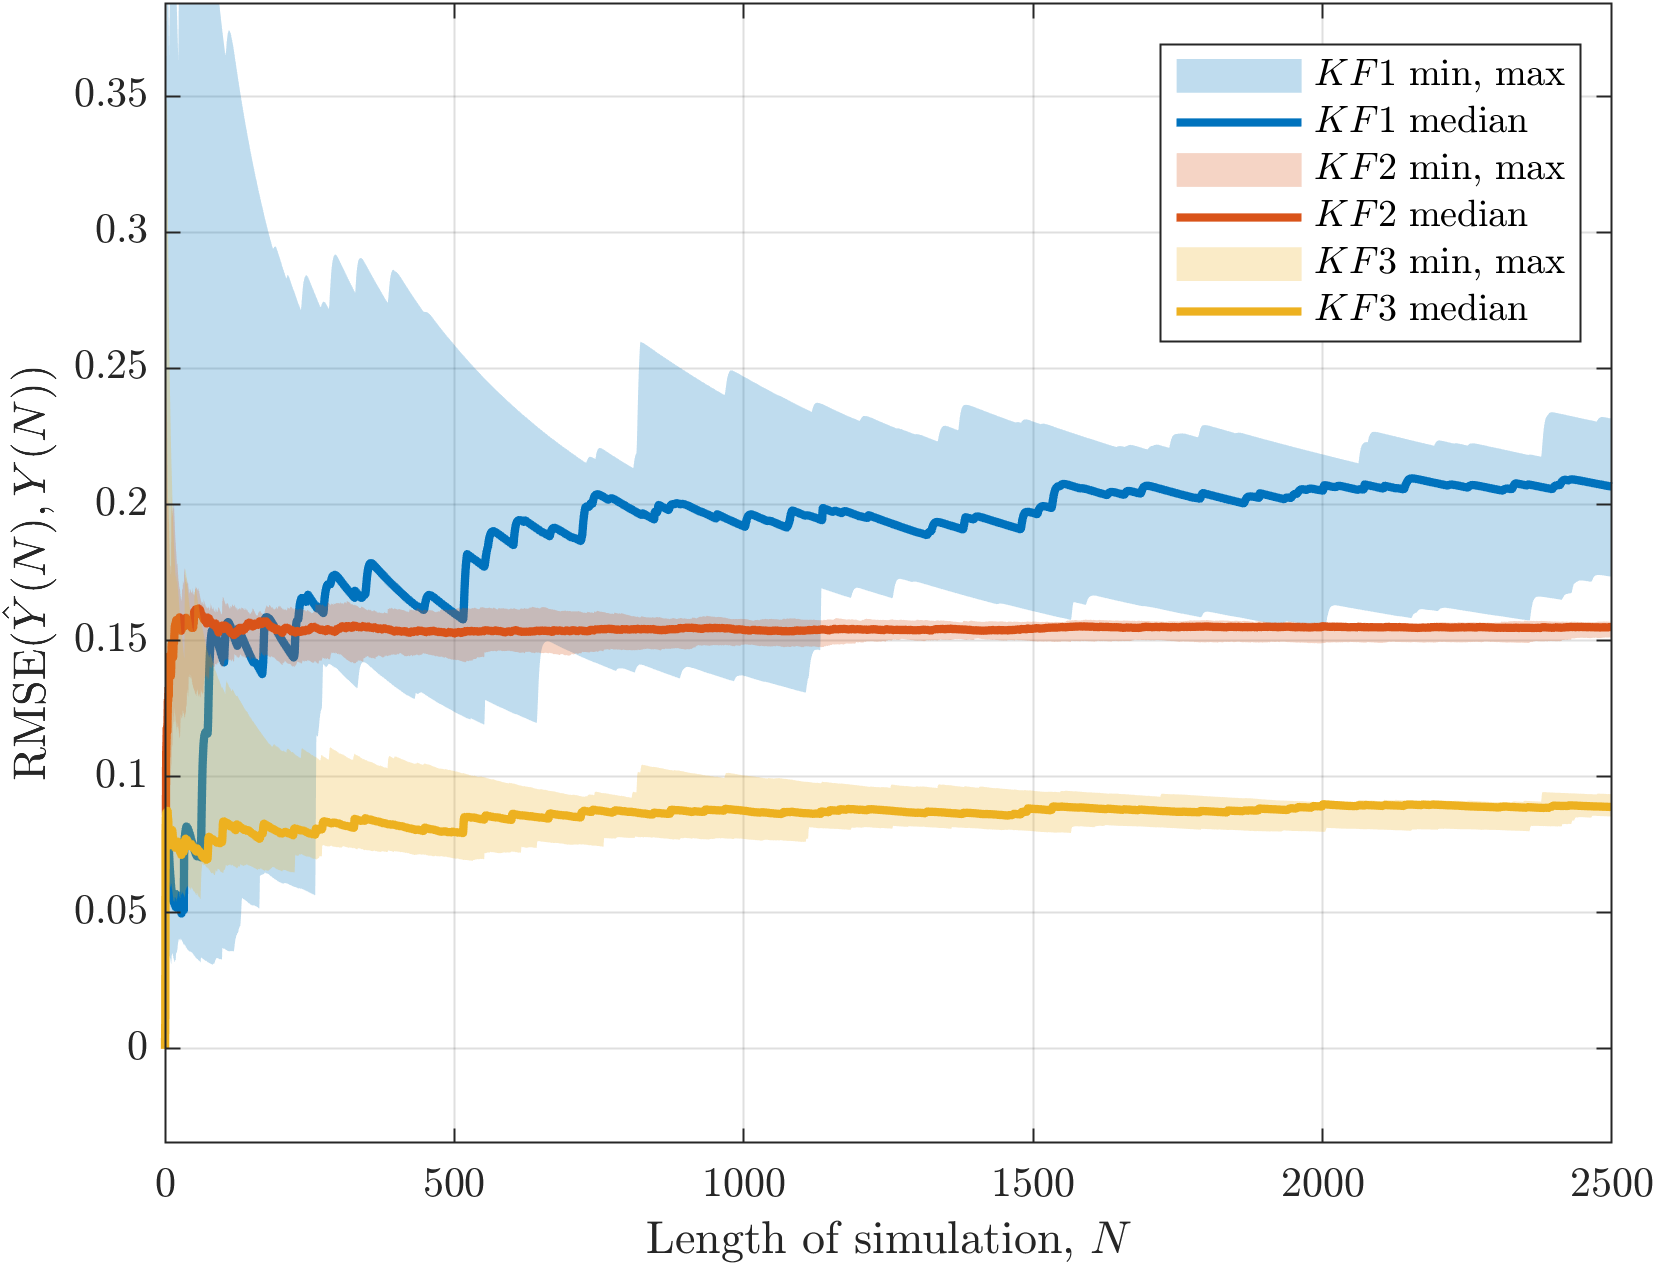
\includegraphics[width=14cm]{images/rod_obs_sim1_3KF_seed_crmse_statsplot.png}  % use png here
	\caption{Effect of random variables on the \gls{RMSE} results.}
	\label{fig:rod-obs-sim-1-3KF-seed-crmse-statsplot}
\end{figure}  %TODO: This needs updating because simulations are old.  Also figures in text.

As expected, the differences in the results due to \gls{PRNG} initialization decrease as the simulation duration increases. However, the magnitude of the differences is not the same for each observer. The \gls{RMSE} values of KF1, which has the lowest gain, are more sensitive to the random initialization than those of the other two filters. Therefore it is not possible to estimate the expected value of the \gls{RMSE} of KF1 from a single simulation of this duration---a longer simulation or a larger number of simulations would be needed. On the other hand, the variations in the \gls{RMSE}s of KF2 and KF3 are significantly lower. After the full length of the simulations ($N=2500$), the \gls{RMSE} of KF2 is between -0.0039 (-2.5\%) and 0.0019 (1.3\%) of the median value, which is $0.1550$.  That of KF3 is between -0.0035 (-4.0\%) / 0.0047 (5.3\%) of the median, which is 0.0889.  Therefore it is reasonable to conclude that the \gls{RMSE} of KF3 is consistently about 0.05 lower than that of KF2. Note that the \gls{RMSE}s of KF2 and KF3 reported in Section \ref{sec:sim-obs-lin-1} are 0.0935 and 0.0672. These values are both within the minimum and maximum values of this sensitivity analysis.
%TODO: The simulation results above need checking/updating.

A similar sensitivity analysis was carried out on the results of the Kalman filter tuning shown in Figure \ref{eq:sim-sys-siso-KF3-Q}, where KF3 was tuned using a set of 5000 input-output samples from the system. Figure \ref{fig:sim-sys-siso-KF3-sensitivity} shows the variation in this result when ten different sets of pseudo-random simulation data are used.  Although there is considerable variation in the \gls{RMSE} values for each parameter value, the best overall choice of $\sigma_{w_p}^2$ to achieve the lowest average error across all 10 simulations was found to be the same as that of the single simulation (0.01).
\begin{figure}[htp]
	\centering
	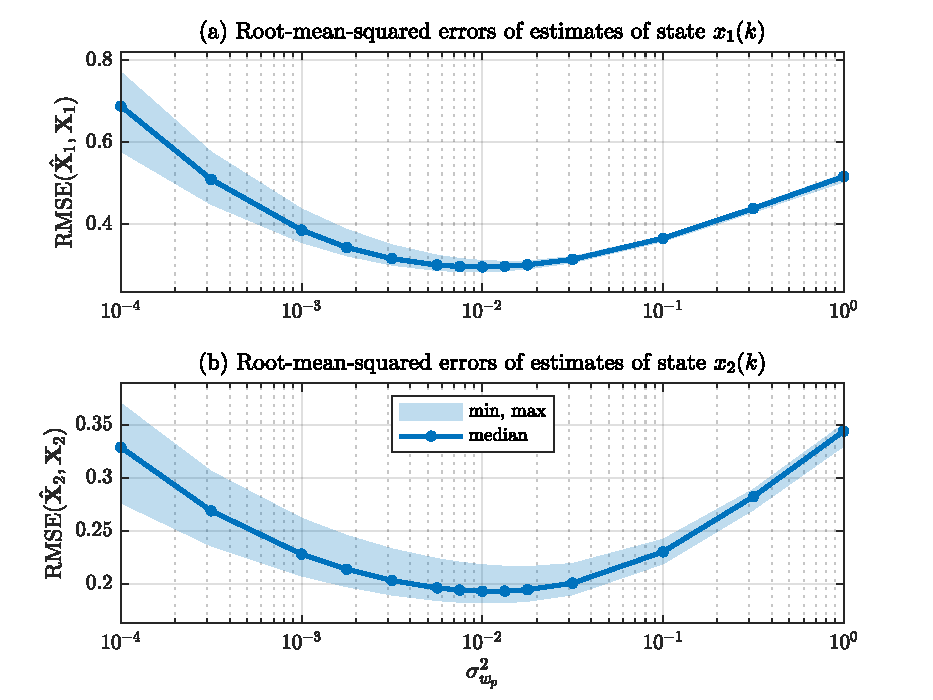
\includegraphics[width=14cm]{images/rod_obs_sim1_3KF_Q_statplot.pdf}
	\caption{Sensitivity of Kalman filter tuning – SISO system}
	\label{fig:sim-sys-siso-KF3-sensitivity}
\end{figure}

Figure \ref{fig:sim-sys-2x2-KF3-tuning-sens} shows the results of a similar sensitivity analysis on the results presented in Figure \ref{fig:sim-sys-2x2-KF3-tuning}.

\begin{figure}[htp]
	\centering
	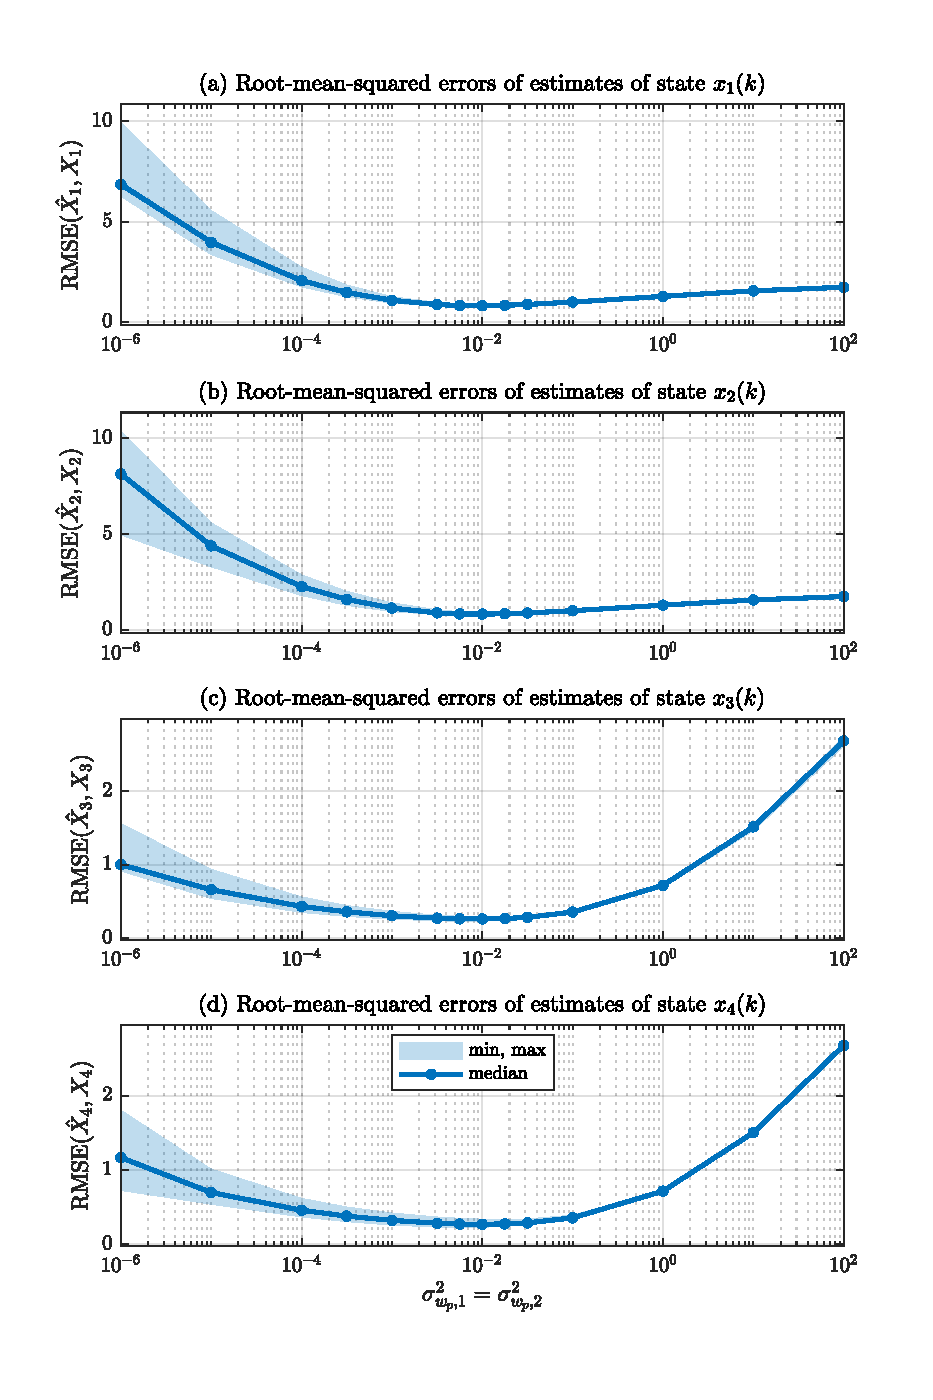
\includegraphics[width=14cm]{images/rod_obs_sim3_3KF_Q_statplot.pdf}
	\caption{Sensitivity of Kalman filter tuning – $2\times2$ system}
	\label{fig:sim-sys-2x2-KF3-tuning-sens}
\end{figure}

